\documentclass[border=10pt]{standalone}

\usepackage{tikz}
\usepackage{tikzsymbols}
\usetikzlibrary{calc,patterns,shapes.geometric}

\def\centerarc[#1](#2)(#3:#4:#5){\draw[#1] ($(#2)+({#5*cos(#3)},{#5*sin(#3)})$) arc (#3:#4:#5);}

\begin{document}
	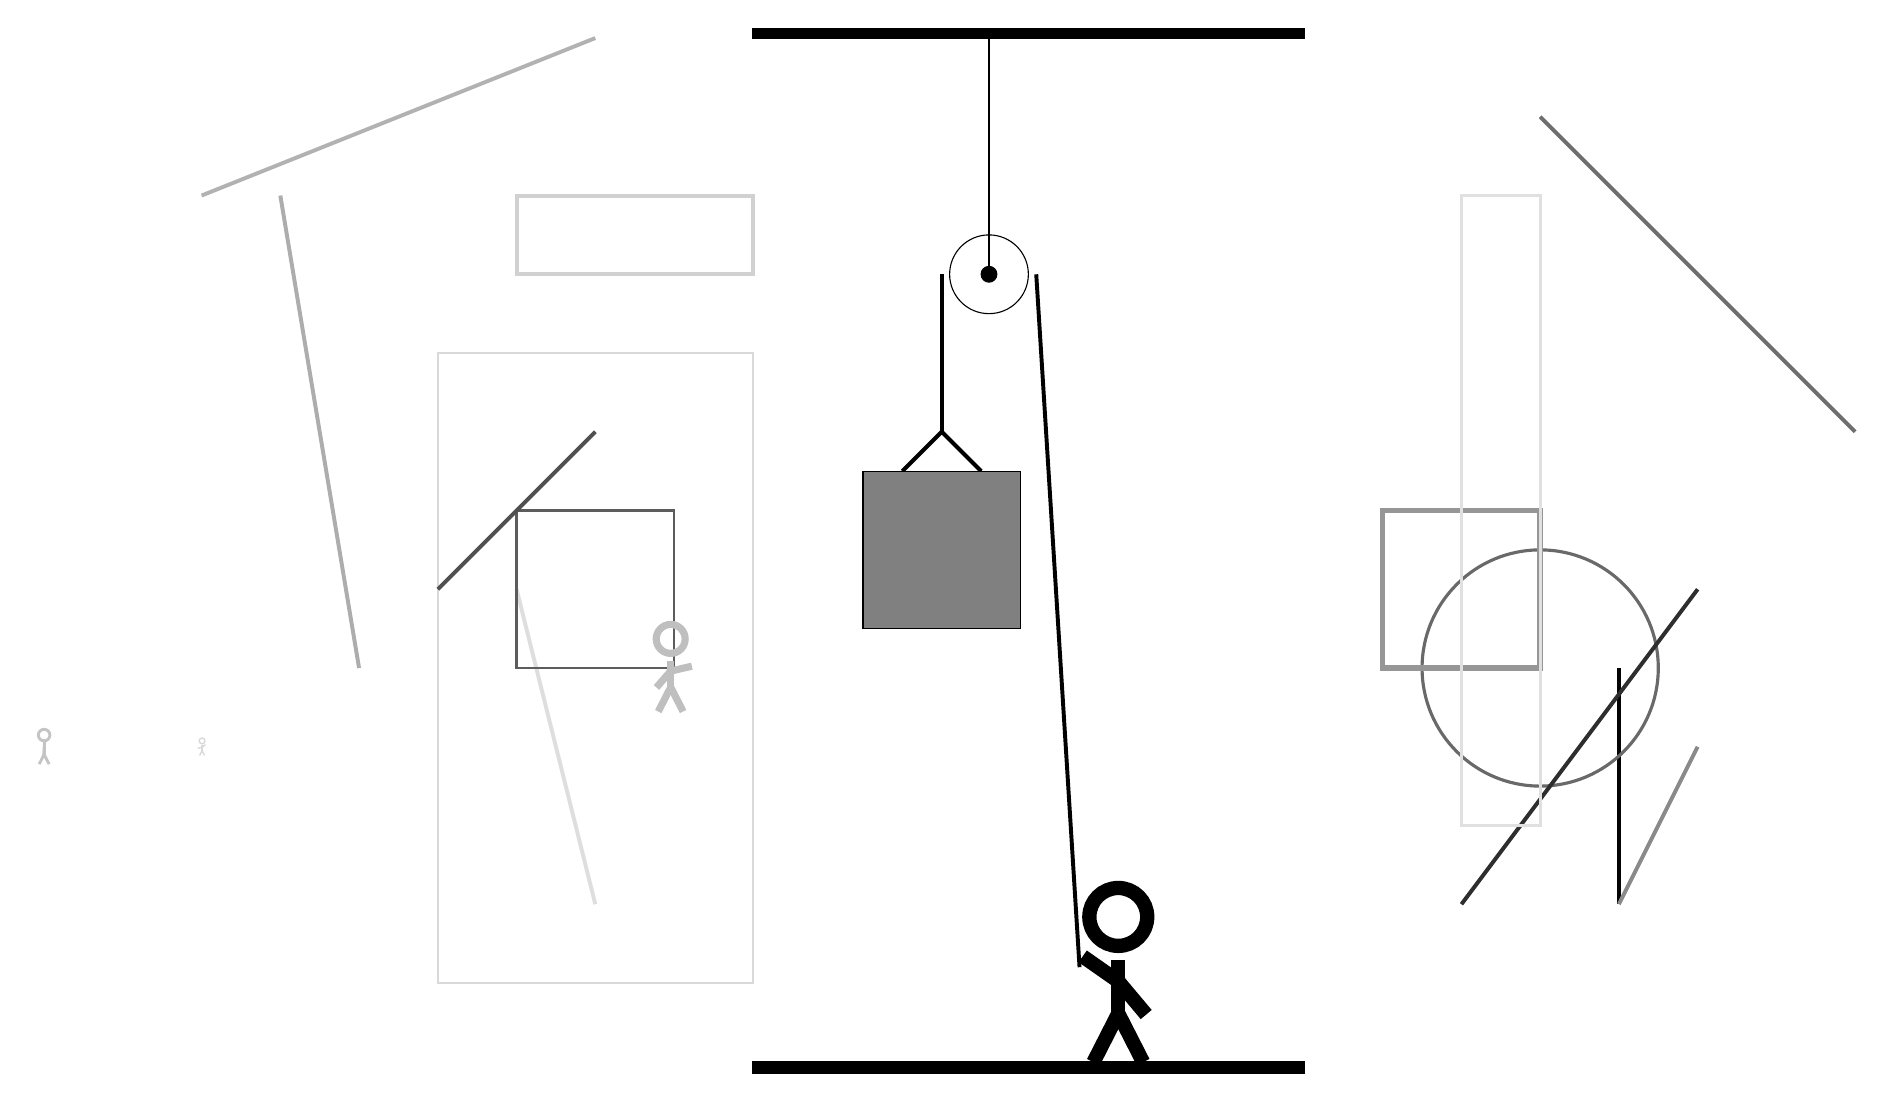
\begin{tikzpicture}
		%%%%% START %%%%%
		
		\draw[fill=black] (-2, 10) rectangle (5, 10.125);
		
		\draw (1, 7) circle (0.5);
		\draw[fill=black] (1, 7) circle (0.1);
		\draw (1, 10) -- (1, 7);
		
		\draw[line width=0.5mm] (-0.1, 4.5) -- (0.4, 5.0) -- (0.9, 4.5);
		\draw[fill=black!50] (-0.6, 4.5) rectangle (1.4, 2.5);
		
		\draw[line width=0.5mm] (0.4, 7) -- (0.4, 5.0);
		\centerarc[line width=0.5mm](1, 7)(0:180:0.6);
		\draw[line width=0.5mm](1.6, 7) -- (2.15, -1.8);
		
		\draw[line width=0.5mm, color=black!99](9, -1) -- (9, 2);
		
		\draw[line width=0.5mm, color=black!46](9, -1) -- (10, 1);
		\node[line width=0.7mm, color=black!15] at (-9, 1) {\Strichmaxerl[1][11][40]};
		\draw[line width=0.5mm, color=black!13](-4, -1) -- (-5, 3);
		
		\draw [line width=0.4mm, color=black!59](8, 2) circle (1.5);
		
		\draw[line width=0.5mm, color=black!57](8, 9) -- (12, 5);
		
		\node[line width=0.5mm, color=black!23] at (-11, 1) {\Strichmaxerl[2][86][86]};
		
		\draw[line width=0.3mm, color=black!64] (-3, 4) rectangle (-5, 2);
		\draw[line width=0.2mm, color=black!15] (-2, 6) rectangle (-6, -2);
		
		\draw[line width=0.5mm, color=black!30](-4, 10) -- (-9, 8);
		\draw[line width=0.7mm, color=black!41] (6, 2) rectangle (8, 4);
		\draw[line width=0.5mm, color=black!69](-6, 3) -- (-4, 5);
		\draw[line width=0.5mm, color=black!82](7, -1) -- (10, 3);
		\node[line width=0.6mm, color=black!25] at (-3, 2) {\Strichmaxerl[5][49][13]};
		\draw[line width=0.4mm, color=black!12] (7, 0) rectangle (8, 8);
		\draw[line width=0.5mm, color=black!18] (-2, 8) rectangle (-5, 7);
		\draw[line width=0.5mm, color=black!32](-7, 2) -- (-8, 8);
		
		
		\node at (2.6, -1.9) {\Strichmaxerl[10][-35][-50]};
		
		\draw[fill=black] (-2, -3) rectangle (5, -3.15);
		
		%%%%% END %%%%%
	\end{tikzpicture}
\end{document}